\documentclass[10pt, a4paper, italian]{article}
\usepackage[T1]{fontenc}
\usepackage[utf8]{inputenc}
\usepackage{amsmath, amssymb, amsthm, thmtools, amsfonts, mathtools}
\usepackage{nicefrac}
\usepackage{calc}
\usepackage[pdftex, hyperindex, plainpages=false]{hyperref}
\usepackage[nameinlink]{cleveref} %load before classicthesis (clash)
%\usepackage[nochapters,pdfspacing]{classicthesis}
\usepackage{siunitx}
\usepackage[siunitx]{circuitikz}

\usepackage[a4paper]{geometry}
\usepackage{float}
\usepackage{mdframed}
\usepackage{titling}
\usepackage{booktabs}
\usepackage{graphicx}
\usepackage{caption, subcaption}
\usepackage{xcolor}
\usepackage[italian]{babel}
\usepackage{pgfplots}
\usepackage{listings}
%\usepackage{lmodern}
\usepackage{url}
\usepackage{enumitem}
\usepackage{tikz} %loads after classicthesis (xcolor incompat)

% lets graphicx know path where figures to be included are found
\graphicspath{{../figs/}}
\makeatletter
\def\input@path{{../figs/}}
%or: \def\input@path{{/path/to/folder/}{/path/to/other/folder/}}
\makeatother

% tikz pgf plots setup
\usepgfplotslibrary{external}
\pgfplotsset{compat=1.15}
%\tikzexternalize

% spaces and significant digits/figures for measurements
\sisetup{free-standing-units, space-before-unit, number-unit-product = \;,
scientific-notation = false, round-mode = figures, round-precision = 1,}

% turns all (hyperlinked) references black [default is blue]
\hypersetup{
	linktoc=all,
	colorlinks=true,
	linkcolor=black
}

% code listings config
%\lstset{
%language=Python,
%basicstyle=\ttfamily,
%columns=fullflexible,
%keepspaces=true,
%}

% mdframed (for boxed text) configuration
\mdfsetup{linewidth=0.6pt}

% Default fixed font does not support bold face
\DeclareFixedFont{\ttb}{T1}{txtt}{bx}{n}{12} % for bold
\DeclareFixedFont{\ttm}{T1}{txtt}{m}{n}{12}  % for normal

% Custom colors
\usepackage{color}
\definecolor{deepblue}{rgb}{0,0,0.5}
\definecolor{deepred}{rgb}{0.6,0,0}
\definecolor{deepgreen}{rgb}{0,0.5,0}

% Commands 
\newcommand{\executeiffilenewer}[3]{%
	\ifnum\pdfstrcmp{\pdffilemoddate{#1}}%
		{\pdffilemoddate{#2}}>0%
	{\immediate\write18{#3}}\fi%
}
% input .svg --> .pdf_tex graphs
%\newcommand{\includesvg}[1]{%
%	\executeiffilenewer{#1.svg}{#1.pdf}%
%	{inkscape -z -D --file=#1.svg %
%	--export-pdf=#1.pdf --export-latex}%
%	\input{#1.pdf_tex}%
%}
% Thanks UniPi's Department of Physics E. Fermi
\newcommand{\thanksdf}{(\thanks{Dipartimento di Fisica E.~Fermi,%
Universit\`a di Pisa - Pisa, Italy.}\;)}

% hyperlink to email address
\newcommand{\mail}[1]{\href{mailto:#1}{\textsf{#1}}}

% \vec for bold vectors, instead of overarrows (now "\arrvec")
\let\arrvec=\vec
\renewcommand{\vec}[1]{\boldsymbol #1}
% replaces straight phi with slanted phi
\renewcommand{\phi}{\varphi}
% replaces straight eps with curved epsilon
\newcommand{\eps}{\varepsilon}
% abbreviation for (sub_/super^)scripts of \lim, \sum,... in inline math
\newcommand{\ds}{\displaystyle}

% blackboard/number set letters
\newcommand{\CC}{\mathbb C}
\newcommand{\HH}{\mathbb H}
\newcommand{\KK}{\mathbb K}
\newcommand{\NN}{\mathbb N}
\newcommand{\PP}{\mathbb P}
\newcommand{\QQ}{\mathbb Q}
\newcommand{\RR}{\mathbb R}
\newcommand{\ZZ}{\mathbb Z}

\newcommand{\Abs}[1]{{\left\Vert #1\right\Vert}}
\newcommand{\enclose}[1]{{\left( #1 \right)}}
\newcommand{\Enclose}[1]{{\left[ #1 \right]}}
\newcommand{\floor}[1]{\left\lfloor #1 \right\rfloor}
\newcommand{\ceil}[1]{\left\lceil #1 \right\rceil}
\newcommand{\To}{\rightrightarrows}

% Math operators
\DeclareMathOperator{\divergence}{div}
\renewcommand{\div}{\divergence}
\DeclareMathOperator{\Imaginarypart}{Im}
\renewcommand{\Im}{\Imaginarypart}
\DeclareMathOperator{\Realpart}{Re}
\renewcommand{\Re}{\Realpart}
%\DeclareMathOperator{\arg}{arg}
\DeclareMathOperator{\tg}{tg}
\DeclareMathOperator{\arctg}{arctg}
\DeclareMathOperator{\settsinh}{settsinh}
\DeclareMathOperator{\settcosh}{settcosh}
\DeclareMathOperator{\tr}{tr}
\DeclareMathOperator{\im}{im}
\DeclareMathOperator{\sgn}{sgn}
\DeclareMathOperator{\diag}{diag}

\DeclarePairedDelimiter{\norm}{\lVert}{\rVert}
\DeclarePairedDelimiter{\scalar}{\langle}{\rangle}

% Logarithm with arbitrary base.
% -> log_10
\newcommand{\llog}[1][10]{\log_{#1}}

% Absolute value.
% -> |x|
\newcommand{\abs}[1]{\left| #1 \right|}

% Powers.
% -> x^a
\newcommand{\power}[2][2]{\left( #2 \right)^{#1}}

% Square.
% -> x^2
\newcommand{\sq}[1]{\power[2]{#1}}

% Expansion of the binomial coefficient.
% -> n1!/(n2!(n1 - n2)!)
\newcommand{\binomexpr}[2]{\frac{#1!}{#2!(#1 - #2)!}}

% Expression evaluation at a given point with square brackets.
% -> [x]_{a}
\newcommand{\at}[2]{\left[ #1\right]_{\makebox[-1pt][l]{${\scriptstyle#2}$}}}

% Expression evaluation in an interval.
% -> [x] _{a}^{b}
\newcommand{\eval}[3]{\left.#1%
  \right|_{\makebox[-1pt][l]{${\scriptstyle#2}$}}^{\makebox[-1pt][l]{${\scriptstyle#3}$}}}

% Upright d in math mode (for differentials).
% -> d
\newcommand{\ud}{\mathrm{d}}

% Differential.
% -> dx
\newcommand{\diff}[1][x]{\,\ud{#1}}

% Base command for defining derivatives.
% -> df/dx or d^kf/dx^k
\newcommand{\basederivative}[4][]{%
  \displaystyle%
  \ifx\\#1\\\frac{#4#2}{#4#3}%
  \else%
  \frac{#4^#1#2}{#4#3^#1}%
  \fi%
}

% Total derivative.
% -> df/dx(x) or d^kf/dx^k(x)
\newcommand{\td}[4][]{%
  \basederivative[#1]{#2}{#3}{\ud}%
  \ifx\\#4\\%
  \else%
  \mkern-4mu\left(#4\right)%
  \fi%
}

% Partial derivative.
% -> df/dx(x) or d^kf/dx^k(x)
\newcommand{\pd}[4][]{%
  \basederivative[#1]{#2}{#3}{\partial}%
  \ifx\\#4\\%
  \else%
  \mkern-4mu\left(#4\right)%
  \fi%
}

\newcommand{\intinf}{\int_{-\infty}^{\infty}\!\!\!}

\newcommand{\cinterval}[2]{\left[\, #1,~#2 \,\right]}

\newcommand{\linterval}[2]{\left[\, #1,~#2 \,\right)}

\newcommand{\rinterval}[2]{\left(\, #1,~#2 \,\right]}

\newcommand{\ointerval}[2]{\left(\, #1,~#2 \,\right)}

\newcommand{\prob}[1]{\displaystyle P\left(#1\right)}

\newcommand{\pvalue}{\emph{$p$-value}}

\newcommand{\cond}{\,|\,}

\newcommand{\expect}[1]{\displaystyle E\left[#1\right]}

\newcommand{\mom}[2][]{\displaystyle {\cal M}_{#2}\ifx\\#1\\\else(#1)\fi}

\newcommand{\momalg}[1]{\displaystyle \lambda_{#1}}

\newcommand{\momcen}[1]{\displaystyle \mu_{#1}}

\newcommand{\skewness}{\displaystyle \gamma_1}

\newcommand{\kurtosis}{\displaystyle \gamma_2}

\newcommand{\charf}[1][x]{\phi_{#1}}

\newcommand{\momgenf}[1][x]{M_{#1}}

\newcommand{\fwhm}{{\scriptstyle \textsc{FWHM}}}

\newcommand{\hwhm}{{\scriptstyle \textsc{HWHM}}}

\newcommand{\median}{\mu_{\nicefrac{1}{2}}}

\newcommand{\var}[1]{\ensuremath{\text{Var}\left(#1\right)}}

\newcommand{\cov}[2]{\ensuremath{\text{Cov}\left(#1, #2\right)}}

\newcommand{\corr}[2]{\ensuremath{\text{Corr}\left(#1, #2\right)}}

\newcommand{\like}{\mathcal L}

\newcommand{\likelihood}[2][]{\like\ifx\\#2\\\else(#2\ifx\\#1\\\else;#1\fi)\fi}

\newcommand{\chisq}{\ensuremath{\chi^2}}

\newcommand{\chisquare}[2][]{\chisq\ifx\\#2\\\else(#2\ifx\\#1\\\else;#1\fi)\fi}

\newcommand{\loglikelihood}[2][]{\log\likelihood[#1]{#2}}

\newcommand{\pdf}[3][]{#2(#3\ifx\\#1\\\else;#1\fi)}

\newcommand{\binomialpdf}[2][]{\pdf[#1]{\mathcal B}{#2}}

\newcommand{\multinomialpdf}[2][]{\pdf[#1]{\mathcal M}{#2}}

\newcommand{\poissonpdf}[2][]{\pdf[#1]{\mathcal P}{#2}}

\newcommand{\uniformpdf}[2][]{\pdf[#1]{u}{#2}}

\newcommand{\exponentialpdf}[2][]{\pdf[#1]{\varepsilon}{#2}}

\newcommand{\gausspdf}[2][]{\pdf[#1]{N}{#2}}

\newcommand{\chisquarepdf}[2][]{\pdf[#1]{\wp}{#2}}

\newcommand{\cauchypdf}[2][]{\pdf[#1]{c}{#2}}

\newcommand{\erf}[1]{\ensuremath{\text{erf}\left(#1\right)}}

\newcommand{\dccases}[4][]{#2 \ifx\\#2\\\else=\fi %
  \begin{cases}
    \displaystyle #3 & \text{per variabili discrete}\\
    \displaystyle #4 & \text{per variabili continue}#1
  \end{cases}
}
% sub/super-scriptable for all symbol as math operator 
\newcommand\Scaleforall[1]{\vcenter{\hbox{\scalefont{#1}$\forall$}}}

\DeclareMathOperator*\forevery{%
  \vphantom\sum
  \mathchoice{\Scaleforall{2}}{\Scaleforall{1.4}}{\Scaleforall{1}}{\Scaleforall{0.75}}}
\geometry{left=2cm, right=2cm, top=2cm, bottom=2cm}

% makes all hyperlinks the same color as text
\hypersetup{
	linktoc=all,
	colorlinks=false,
	linkcolor=black
	}
% lets graphicx know path where figures to be included are found
\graphicspath{{../figs/}}

\author{Gruppo 1.AC \\ Matteo Rossi, Bernardo Tomelleri}
\title{Es10: Misura del rapporto carica-massa dell'elettrone $e/m_e$}
\begin{document}
\date{\today}
\maketitle

%=======================
\section{Scopo dell'esperienza}
Si vuole misurare il rapporto $e/m$ attraverso la misura del raggio di
curvatura della traiettoria circolare di un fascio di elettroni immersi in un
campo magnetico uniforme (generato da bobine in configurazione di Helmholtz)
accelerati da una differenza di potenziale nota.

\begin{figure}[htbp]
    \centering
	%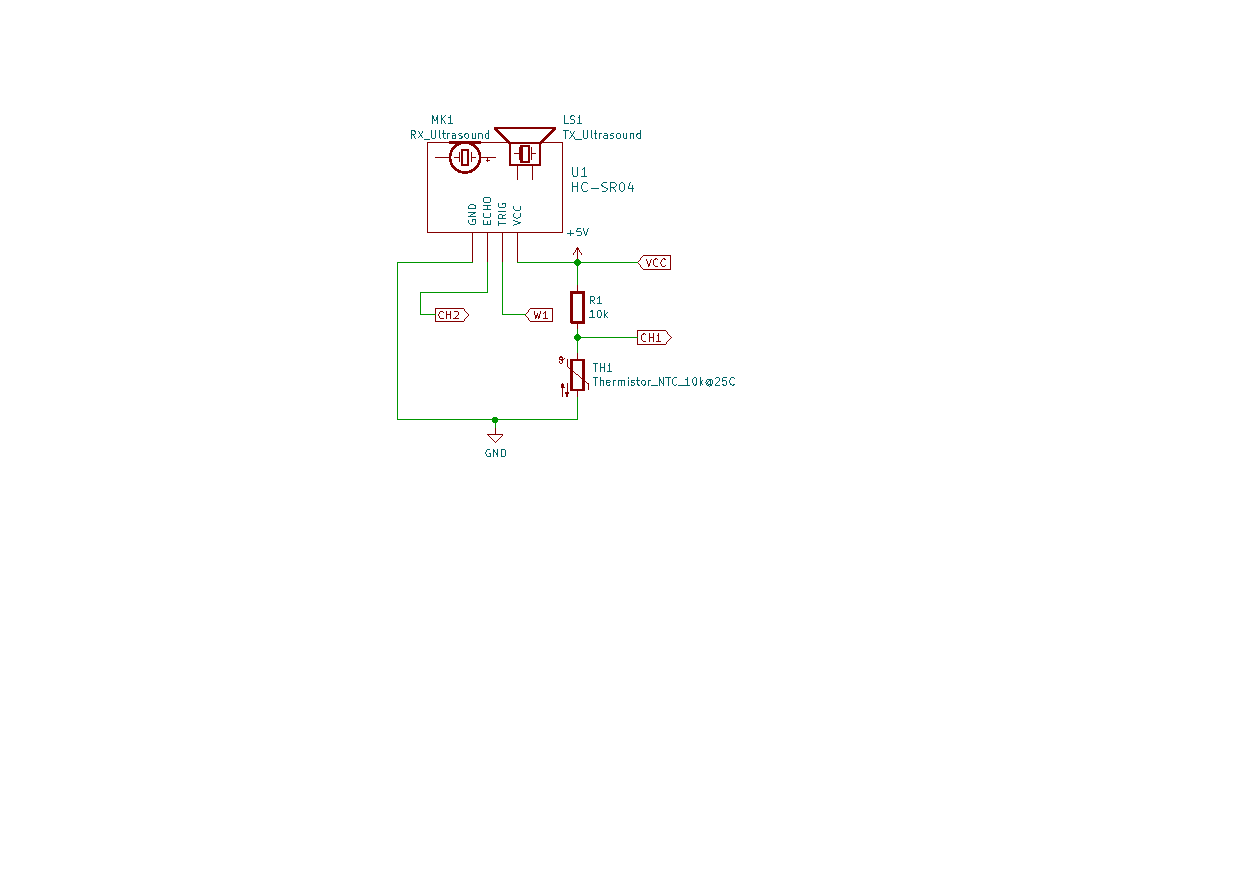
\includegraphics[scale=0.7]{schm}
    \caption{Schema dei circuiti di emissione e rilevazione di intensità
    luminosa.
    \label{schm: mesctrl}}
\end{figure}

\section{Metodo di misura}
Consideriamo il campo magnetico prodotto da due bobine coassiali di raggio
medio $r = 15.8 \; \si{c\m}$, costituite da $N = 130$ spire collegate in
serie e percorse da una stessa corrente di intensità $I\ped{coil}$ da noi
controllabile.

Si può calcolare il campo magnetico nella regione vicino al centro di ciascuna
bobina dalla legge di Biot-Savart e, quando queste sono poste ad una distanza
$a = r$ pari al loro raggio -cioè in configurazione di Helmholtz- si può
ricavare un'espressione per il campo totale come sovrapposizione dei due campi
\begin{equation}\label{eq: B-helm}
    B = \frac{\mu_0 N r^2 I\ped{coil}}{\left[r^2 + \left(\dfrac{r}{2}\right)^2
    \right]^\frac{3}{2}} =
    \left(\frac{4}{5}\right)^{\frac{3}{2}} \frac{\mu_{0} N}{r} I\ped{coil}.
\end{equation}
Nel piano parallelo alle spire passante per il punto medio dell'asse
congiungente i centri delle bobine (ovvero il piano della traiettoria degli
elettroni) il campo magnetico è parallelo all'asse $z$ delle spire ed ha
valore massimo della componente lungo lo stesso asse:
\[
Bz\ped{MAX} = 7.40 10^{-4} I\ped{coil}
\]

Un catodo, riscaldato da un filamento incandescente alimentato con una
tensione $V\ped{heat} = \SI{6}{\V}$ emette elettroni per effetto termoionico.
Gli elettroni vengono accelerati da una d.d.p. $V\ped{acc}$ compresa tra 150
e 250 V e, all'uscita dal cannone elettronico urtano gli atomi del gas
rarefatto (He, a pressione di $10^{-1} \; \si{\Pa}$) presente nell'ampolla,
i quali emettono la radiazione che consente di visualizzare il pennello e
misurarne l'orbita.

Una volta liberati dal catodo, nella regione in cui supponiamo assente il
campo elettrico $V\ped{acc}$, per la conservazione dell'energia vale
\begin{equation}\label{eq: T=qV}
    \frac{1}{2} m_{e} v^{2} = e V\ped{acc}
\end{equation}
Per cui, assumendo che il campo magnetico sia statico e uniforme lungo $z$ e
che il fascio di elettroni abbia velocità ortogonale all'asse delle spire,
ci aspettiamo che gli elettroni rimangano in moto circolare uniforme nel
piano ortogonale $x-y$.

Dalla condizione di moto circolare di raggio $R$ dovuto alla forza di Lorentz
abbiamo che
\[
m_{e} \frac{v^2}{R} = e v B \implies v = \frac{e}{m_e} B R
\]
Combinando l'~\cref{eq: T=qV} con la precedente troviamo
\[
v^2 = 2 V\ped{acc} \frac{e}{m_e} \implies \left(\frac{e}{m_e} B R\right)^2 =
2 V\ped{acc} \frac{e}{m_e}
\]
Da cui otteniamo l'equazione tramite cui vogliamo stimare il rapporto
\begin{equation}\label{eq: fit}
\frac{e}{m_{e}} = \frac{2 \Delta V}{(BR)^2}.
\end{equation}

Dal momento che tutte le variabili nel RHS sono direttamente controllabili
configurando le tensioni di alimentazione e possiamo misurare il raggio
della traiettoria $R$ analizzando (come faremo ad esempio con un fit
circolare) le fotografie del moto nel bulbo.

%=======================
\section{Descrizione delle misure}
\subsection{Orientazione delle bobine rispetto al campo magnetico terrestre}
Usando le due bussole in dotazione e la bussola di un cellulare abbiamo per
prima cosa orientato l'apparato in modo che il campo magnetico generato dalle
bobine fosse nella stessa direzione del cam
\subsection{Mappatura del campo magnetico lungo l'asse delle bobine}

\subsection{Calibrazione dell'apparato per l'acquisizione delle traiettorie}
\label{sec: conv}

%TODO riscrivere
\subsection{Misura del raggio della traiettoria}
Sulle foto sopra menzionate si è effettuato un campionamento dei punti
sull'arco interno e sull'arco esterno. Le coordinate dei pixel così ricavate
sono state interpolate con un \emph{fit} circolare per ottenere una stima del
raggio interno ed esterno. Si è poi assunto come valore efficace del raggio
dell'orbita la media del raggio del cerchio interno e di quello esterno,
e si è attribuito un errore pari alla semi-dispersione degli stessi.
I raggi così ottenuti sono stati poi convertiti in unità fisiche come spiegato
nella~\cref{sec: conv}. \\

\section{Analisi dati e stima del rapporto $e/m$}
La stima del rapporto $ e/m_{e} $ è stata poi ottenuta in due modi diversi:
come media pesata delle singole misure ottenute dalla~\eqref{eq: fit} ed
effettuando un \emph{fit} lineare di $ 2\Delta V $ al variare di
$ (B R)^{2} $ e ottenendo $ e/m_{e} $ dal coefficiente angolare della retta
di \emph{best-fit}.

Prendendo come valori esatti $e = \SI{1.602176634e11}{\coulomb}$ e
$m_{e} = \SI{9.10938370e-31}{\kilogram}$ il valore atteso per il loro
rapporto è
\begin{equation}\label{eq: e-m-exp}
\left(\frac{e}{m_{e}}\right)\ped{exp} = \SI{175.882e9}{\coulomb/\kilogram}
\end{equation}

%=======================
\section{Valutazione degli effetti sistematici}
\subsection{Spessore del pennello elettronico}

\subsection{Dipendenza della stima di $e/m$ dal raggio dell'orbita $R$}

\subsection{Distorsione del bulbo di vetro}

\subsection{Campo magnetico terrestre}

\subsection{Disuniformità del campo magnetico sulla traiettoria}

%=======================
\section*{Conclusioni e commenti finali}
Si è riusciti a dare una misura ragionevole del rapporto carica/massa
dell'elettrone a partire da un'analisi delle fotografie della sua traiettoria
elicoidale in presenza di un campo magnetico uniforme.

%=======================
\section*{Dichiarazione}
I firmatari di questa relazione dichiarano che il contenuto della relazione \`e
originale, con misure effettuate dai membri del gruppo, e che tutti i firmatari
hanno contribuito alla elaborazione della relazione stessa.

%=======================
\begin{thebibliography}{1}
\bibitem{Coope}{I. D. Coope, Circle fitting by linear and nonlinear least
squares, Department of Mathematics, University of Canterbury, Christchurch,
New Zealand, N.60, May, 1992,
\url{https://ir.canterbury.ac.nz/bitstream/handle/10092/11104/coope_report_no69_1992.pdf?sequence=1&isAllowed=y}}
\end{thebibliography}

\end{document}
